\def\myamplitude{0.80}% Amplitude of u2, relative to u1
\def\myphase{0.20} % Phase shift of u2, negatively absolute in pi to u1
\def\myomegaindex{6}% omega, relative to omega0=1 % no stretching of x-axis as x=omega*t
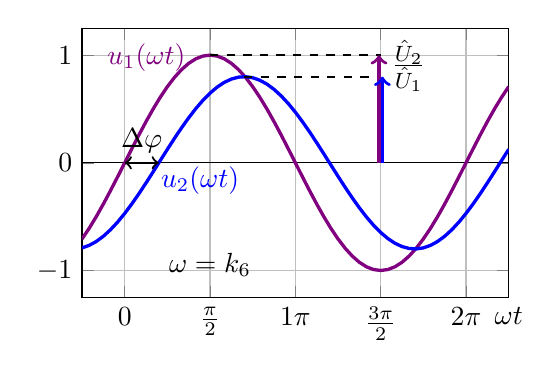
\begin{tikzpicture}
    % invisible boundbox
    %\draw[draw=black](-0.3,-0.125) rectangle (+5.5,+2);
    \begin{axis}[%
        %xlabel={$\omega t$},
        xmin=-0.25, xmax=2.25, % pi
        domain=-0.25:2.25, 
        ymin=-1.25, ymax=1.25,
        samples=61,
        %axis x line=center,
        width=7cm,
        height=5cm,
        xtick={0,0.5,1,1.5,2,2.25},
        xticklabels={0,$\frac{\pi}{2}$,$1\pi$,$\frac{3\pi}{2}$,$2\pi$,$\omega t$},
        grid=both,
        ]
        % x-axis
        \addplot[mark=none,thin,color=black]coordinates{(-0.25,0)(2.25,0)}; % x-axis
        % plots + labels
        \addplot[mark=none,very thick,color=violet]{1.0*sin(deg(x*pi))}  node[pos=0.3,anchor=east,xshift=-1pt] {$u_1(\omega t)$};%
        \addplot[mark=none,very thick,color=blue]{\myamplitude*sin(deg(x*pi-\myphase*pi))}  node[pos=0.15,anchor=west,xshift=1pt] {$u_2(\omega t)$};%
        % phase shift and amplitude change
        \addplot[mark=none,thick,<->]coordinates{(0,0)(\myphase,0)} node[pos=0.5,anchor=south] {$\Delta\varphi$};% Phasenverschiebung
        \addplot[mark=none,thick,dashed]            coordinates{(0.5,1)(1.5,1)};% Amplitude u1
        \addplot[mark=none,thick,dashed]            coordinates{(0.5+\myphase,\myamplitude)(1.5,\myamplitude)};% Amplitude u2
        \addplot[mark=none,very thick,->,color=violet] coordinates{(1.5-0.01,0)(1.5-0.01,1)};
        \addplot[mark=none,very thick,->,color=blue]coordinates{(1.5+0.01,0)(1.5+0.01,\myamplitude)};
        \addplot[mark=none,very thick,draw=none]    coordinates{(1.5,\myamplitude)   (1.5,1)} node[pos=0.5,anchor=west] {\large{$\frac{\hat{U}_2}{\hat{U}_1}$}}; % increase fontsize with \large
        % node omega index
        \addplot[mark=none,draw=none]coordinates{(0.5,-0.95)} node {$\omega=k_{\myomegaindex}$};% omega index
        
    \end{axis}%
\end{tikzpicture}%
